\documentclass[
    NAME={Dr. Helga Ingimundardóttir},
    EMAIL={helgaingim@hi.is},
    FACULTY={Industrial Engineering},
    TITLE={Local and Global Optimization},
    SUBTITLE={Understanding Optima in Complex Landscapes},
    SEMINAR={VÉL113F},
    DATE={Design and Optimization},
    WIDE=true
]{../HI-latex/hi-beamer}
\let\oldframe\frame
\renewcommand\frame[1][allowframebreaks]{\oldframe[#1]}

% Define new commands for nested itemize
\newcommand{\bi}{\begin{itemize}
                     \item}
\newcommand{\ei}{\end{itemize}}

\usepackage{IEEEtrantools}

\usepackage{algorithm}
\usepackage{algpseudocode}

% use mathbf instead of vec
\renewcommand{\vec}[1]{\ifmmode\text{\boldmath$#1$}\else\textbf{#1}\fi}
\newcommand{\mat}[1]{\mathbf{#1}}

\begin{document}

    \begin{frame}{Introduction}
        Delve into the dynamics of optimization landscapes, differentiating between local optima and the overarching
        global optimum, and the techniques to approach each.
    \end{frame}

    \begin{frame}{Mathematical Programming}
        \small

        \emph{Calculus Methods}: Using mathematical tools to solve problems involving change and motion.
        \bi Determining the fastest moment a car was going during a trip. \ei

        \emph{Calculus of Variations}: A field of mathematical analysis that deals with maximizing or minimizing functionals.
        \bi Finding the shortest path a beam of light can take to reflect off a surface. \ei

        \emph{Nonlinear Programming}: Optimizing functions that are not straight lines.
        \bi Maximizing profit when the production cost changes as you produce more. \ei

        \emph{Geometric Programming}: Optimization technique based on polynomial equations.
        \bi Designing a soda can with the least material but a specific volume. \ei

        \emph{Quadratic Programming}: Optimizing quadratic functions, which are polynomials of degree 2.
        \bi Minimizing the cost of production given certain constraints. \ei

        \emph{Linear Programming}: A method to achieve the best outcome in a mathematical model whose requirements
        are represented by linear relationships.
        \bi Finding the best combination of products to manufacture to maximize profit. \ei

        \emph{Dynamic Programming}: Breaking down a problem into simpler parts and solving each part only once.
        \bi Figuring out the most efficient way to store data to minimize retrieval time. \ei

        \emph{Integer Programming}: Optimization where some of the variables are restricted to integer values.
        \bi Deciding the number of buses a school should deploy, as you can't have a fraction of a bus. \ei

        \emph{Stochastic Programming}: Making decisions in the face of uncertainty.
        \bi Planning for the future stock of a store when future demand is uncertain. \ei
        \framebreak
        \emph{Separable Programming}: A nonlinear program where the objective and constraint functions are separable.
        \bi Maximizing crop yield by optimizing the amount of water and fertilizer used when the effects of
        each are independent. \ei

        \emph{Multi-objective Programming}: Making decisions while considering multiple goals simultaneously.
        \bi Designing a product that's both low-cost and high-quality. \ei

        \emph{Network Methods, CPM and PERT}: Tools for project planning and control.
        \bi Organizing tasks when building a house to ensure it's done efficiently and on time. \ei

        \emph{Game Theory}: Studying mathematical models of strategic interactions among rational decision-makers.
        \bi Two businesses deciding on the price of a product, considering what the other might charge. \ei
    \end{frame}

    \begin{frame}{Stochastic and Statistical Methods}
        \small
        \emph{Stochastic Processing Techniques}: Techniques to handle processes that involve uncertainty.
        \bi Predicting stock prices based on past fluctuations.\ei

        \emph{Statistical Decision Theory}: Making decisions using data analysis.
        \bi Choosing to launch a product based on customer survey data.\ei

        \emph{Markov Processes}: Processes where the next state depends only on the current state.
        \bi Predicting tomorrow's weather based on today's.\ei

        \emph{Queuing Theory}: Studying the behavior of waiting lines.
        \bi Optimizing supermarket cashiers to reduce wait times.\ei

        \emph{Renewal Theory}: Statistics of the time to events in processes.
        \bi Predicting machine failure based on past breakdowns.\ei

        \emph{Simulation Methods}: Imitating a real-world process using a model.
        \bi Predicting drug spread using a computer model.\ei

        \emph{Reliability Theory}: Predicting and enhancing system durability.
        \bi Determining average lifespan of a car part.\ei

        \emph{Regression Analysis}: Examining relationships between variables.
        \bi Determining sales relation to advertising.\ei

        \emph{Cluster Analysis \& Pattern Recognition}: Grouping based on similarities.
        \bi Grouping customers by buying habits.\ei

        \emph{Design of Experiments}: Planning experiments to get valid data.
        \bi Testing if new fertilizer improves growth.\ei

        \emph{Discriminant Analysis/Factor Analysis}: Breaking down data into core influences.
        \bi Understanding factors influencing grades.\ei
    \end{frame}

    \begin{frame}{Modern Optimization Techniques}
        \small
        \emph{Genetic Algorithms}: Optimization using natural selection principles.
        \bi Finding best airplane wing design by "evolving" designs. \ei

        \emph{Simulated Annealing}: Probabilistic optimization mimicking the annealing process.
        \bi Optimizing delivery routes. \ei

        \emph{Ant Colony Optimization}: Optimization using ant behavior.
        \bi Optimizing city traffic flow.\ei

        \emph{Particle Swarm Optimization}: Optimization based on flock behavior.
        \bi Adjusting wind turbine design for efficiency.\ei

        \emph{Neural Networks}: Algorithms designed to recognize patterns.
        \bi Recognizing faces in photos.\ei

        \emph{Fuzzy Optimization}: Optimization using fuzzy logic rather than binary.
        \bi Adjusting car heat based on "warm" or "cold".\ei
    \end{frame}

    \begin{frame}{Classification of Optimization Problems}
        \emph{Equations Involved:} Based on the nature of equations.
        \bi Linear vs. Nonlinear equations.\ei

        \emph{Design Variables Values:} Based on permissible values.
        \bi Discrete variables in selecting warehouse locations.\ei

        \emph{Deterministic Nature:} Based on variables' determinacy.
        \bi Predictable machine outputs vs. unpredictable stock prices.\ei

        \emph{Existence of Constraints:} Whether constraints are present.
        \bi Maximizing revenue with a limited budget.\ei
        \framebreak
        \emph{Design Variables Nature:} Nature of the variables involved.
        \bi Binary choices in a network design.\ei

        \emph{Physical Structure:} Based on the problem's inherent structure.
        \bi Structural engineering optimizations.\ei

        \emph{Separability of Functions:} If functions can be separated.
        \bi Independent departmental budgets in a company. \ei

        \emph{Number of Objectives:} Based on the number of goals.
        \bi Balancing cost, quality, and time in project management. \ei

    \end{frame}


    \begin{frame}{Objective Function: Maximize or Minimize}
        The choice between maximizing and minimizing a function can often be translated by considering the
        function's opposite or a scaled version of the function.

        \begin{columns}
            \begin{column}{0.5\textwidth}
                \centering
                \begin{figure}
                    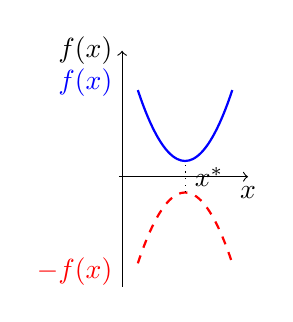
\begin{tikzpicture}[scale=0.4]
                        \draw[->] (-.1,0) -- (4,0) node[anchor=north] {$x$};
                        \draw[->] (0,-3.5) -- (0,4) node[anchor=east] {$f(x)$};
                        \draw[thick, blue] plot[smooth, domain=-1.5:1.5] (2+\x, {0.5+(\x)^2});
                        \draw[thick, red, dashed] plot[smooth, domain=-1.5:1.5] (2+\x, {-.5-(\x)^2});
                        \draw[-,dotted] (2,-.5) -- (2,.5) node[midway, anchor=west] {$x^*$};
                        \node at (0,3) [anchor=east] {\color{blue}$f(x)$};
                        \node at (0,-3) [anchor=east] {\color{red}$-f(x)$};
                    \end{tikzpicture}
                    \caption{$\min_{x} f(x)  \Longleftrightarrow \max_{x} -f(x)$}
                \end{figure}
            \end{column}

            \begin{column}{0.6\textwidth}
                \centering
                \begin{figure}
                    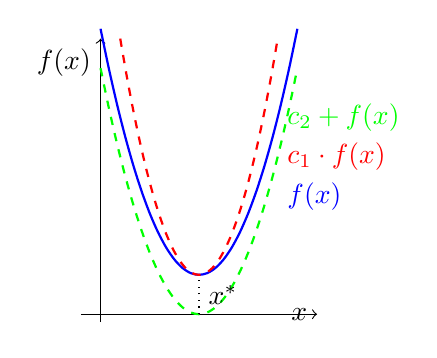
\begin{tikzpicture}[scale=0.5]
                        \draw[->] (-3,0) -- (3,0) node[anchor=east] {$x$};
                        \draw[->] (-2.5,-.2) -- (-2.5,7) node[anchor=north east] {$f(x)$};
                        \draw[thick, blue] plot[smooth, domain=-2.5:2.5] (\x, {1+(\x)^2});
                        \draw[thick, red, dashed] plot[smooth, domain=-2:2] (\x, {1+1.5*(\x)^2});
                        \draw[thick, green, dashed] plot[smooth, domain=-2.5:2.5] (\x, {(\x)^2});
                        \node at (2,4) [anchor=west] {\color{red}$c_1 \cdot f(x)$};
                        \node at (2,3) [anchor=west] {\color{blue}$f(x)$};
                        \node at (2,5) [anchor=west] {\color{green}$c_2 + f(x)$};
                        \draw[-,dotted] (0,0) -- (0,1) node[midway, anchor=west] {$x^*$};
                    \end{tikzpicture}
                    \caption{Scaled $c_1 \cdot f(x)$ and translated $c_2+f(x)$ both retain the original shape.}
                \end{figure}
            \end{column}
        \end{columns}
    \end{frame}

    \begin{frame}{Single Variable Optimization}
        \begin{block}{Single variable optimization with no constraints}
            Determine the value of $x=x^*$ within the interval $[a, b]$ that minimizes the function $f(x)$.
        \end{block}
        \begin{alert}{Necessary Condition}
            If a function $f(x)$ is defined in the interval $a \leq x \leq b$ and has a relative minimum at $x=x^*$, where $a < x^* < b$, and if the derivative $\frac{df(x)}{dx} = f'(x)$ exists as a finite number at $x=x^*$, then $f'(x^*) = 0$.
        \end{alert}
        \begin{columns}
            \begin{column}{0.6\textwidth}
                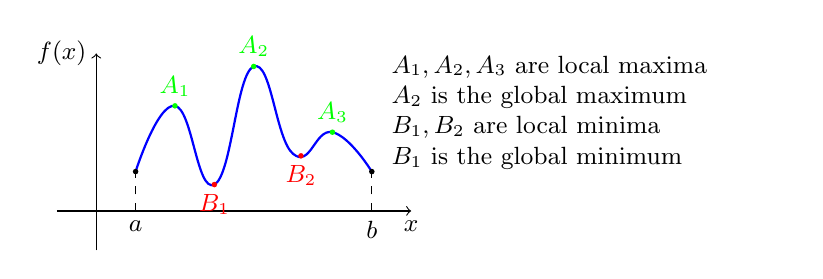
\begin{tikzpicture}[scale=0.5,every node/.style={font=\small}]
                    \draw[->] (-2,1) -- (7,1) node[anchor=north] {$x$};
                    \draw[->] (-1,0) -- (-1,5) node[anchor=east] {$f(x)$};

                    % Drawing the smooth curve
                    \draw[thick, blue, domain=0:4, smooth, tension=.8] plot coordinates {(0,2) (1,3.67) (2,1.67) (3,4.67) (4,2.45) (5,3
                    ) (6,2)};

                    % Maxima points in green
                    \fill[green] (1,3.67) circle (2pt) node[above] {$A_1$};
                    \fill[green] (3,4.67) circle (2pt) node[above] {$A_2$};
                    \fill[green] (5,3) circle (2pt) node[above] {$A_3$};

                    % Minima points in red
                    \fill[red] (2,1.67) circle (2pt) node[below] {$B_1$};
                    \fill[red] (4.2,2.4) circle (2pt) node[below] {$B_2$};

                    % The points a and b
                    \draw[-,dashed] (0,1) -- (0,2) node[at start, below] {$a$};
                    \fill[black] (0,2) circle (2pt);
                    \draw[-,dashed] (6,1) -- (6,2) node[at start, below] {$b$};
                    \fill[black] (6,2) circle (2pt);

                    % Annotations
                    \node[align=left, text width=5cm] at (11.5,3.5) {
                        \( A_1, A_2, A_3 \) are local maxima \\
                        \( A_2 \) is the global maximum \\
                        \( B_1, B_2 \) are local minima \\
                        \( B_1 \) is the global minimum
                    };
                \end{tikzpicture}

            \end{column}
            \begin{column}{0.4\textwidth}
                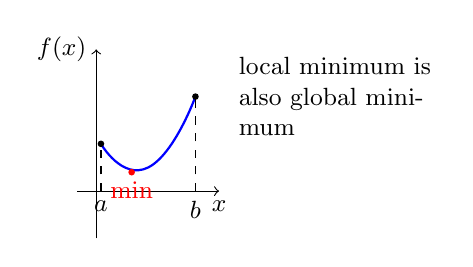
\begin{tikzpicture}[scale=0.6,every node/.style={font=\small}]
                    \draw[->] (-.5,0) -- (2.5,0) node[anchor=north] {$x$};
                    \draw[->] (-.1,-1) -- (-.1,3) node[anchor=east] {$f(x)$};
                    \draw[thick, blue, domain=0:4, smooth, tension=1] plot coordinates {(0,1) (1,0.5) (2,2)};
                    \fill[red] (.65,0.4) circle (2pt) node[anchor=north] {min};
                    \draw[-,dashed] (0,0) -- (0,1) node[at start, below] {$a$};
                    \fill[black] (0,1) circle (2pt);
                    \draw[-,dashed] (2,0) -- (2,2) node[at start, below] {$b$};
                    \fill[black] (2,2) circle (2pt);
                    \node[align=left, text width=2.5cm] at (5,2) {local minimum is also global minimum};
                \end{tikzpicture}
            \end{column}
        \end{columns}

        \begin{block}{Considerations}
            \begin{itemize}
                \item The proof holds even if \(x^*\) is a local maximum.
                \item The derivative's existence at \(x^*\) is not guaranteed for every minimum or maximum.
                \item Extrema at the endpoints of the function's definition interval are not covered.
                \item A zero derivative doesn't guarantee the presence of an extremum; it could be an inflection (or saddle) point.
            \end{itemize}
        \end{block}

        \framebreak
        \begin{block}{Sufficient Condition for Extrema}
            Let's assume the first \(n-1\) derivatives at point \(x^*\) are zero, but the \(n\)th derivative is not zero.

            \begin{itemize}
                \item If the \(n\)th derivative at \(x^*\) is positive and \(n\) is even, then \(f(x^*)\) is a minimum.
                \item If the \(n\)th derivative at \(x^*\) is negative and \(n\) is even, then \(f(x^*)\) is a maximum.
                \item If \(n\) is odd, \(f(x^*)\) is neither a maximum nor a minimum.
            \end{itemize}
        \end{block}

        Think of the even \(n\) as giving the function "another chance" to decide if it's curving up or down. Odd \(n\) means the function hasn't settled into a curve direction.
    \end{frame}

    \begin{frame}{Multivariable Optimization}

        \begin{block}{Multivariable Optimization: Necessity vs. Sufficiency}
            In single-variable optimization, a zero derivative suggests potential extrema. Similarly, in the
            multivariable case, all first partial derivatives should be zero at a stationary point, constituting the
            \emph{necessary condition}. To further discern if it's genuinely a maximum or minimum
            (and not a saddle point), we turn to the Hessian matrix for the \emph{sufficient condition}.
        \end{block}
        Simply put, for a point to be a high or low point in multiple dimensions, the function shouldn't be rising or falling in any of those directions.

        \framebreak
        \begin{alert}{Necessary Condition}
            For a function \(f(\mathbf{x})\) to have an extreme point at \(\mathbf{x} = \mathbf{x^*}\):
            \[
                \frac{\partial f}{\partial x_1}(\mathbf{x^*}) = \frac{\partial f}{\partial x_2}(\mathbf{x^*}) = \dots = \frac{\partial f}{\partial x_n}(\mathbf{x^*}) = 0
            \]
        \end{alert}

        \begin{alert}{Sufficient Condition}
            To determine the nature of a stationary point \(\mathbf{x^*}\) of the function \(f(\mathbf{x})\):
            \begin{itemize}
                \item If the Hessian matrix at \(\mathbf{x^*}\) is positive definite, \(\mathbf{x^*}\) is a local minimum.
                \item If it's negative definite, \(\mathbf{x^*}\) is a local maximum.
            \end{itemize}
            This helps us be certain about the nature of the stationary point.
        \end{alert}

        \framebreak

        \begin{block}{Refresher: The Hessian Matrix}
            The Hessian matrix \(H\) of a function \(f(\mathbf{x})\) is the matrix of its second-order partial derivatives. It provides insight into the curvature of the function:
            \[
                H = \begin{bmatrix}
                        \frac{\partial^2 f}{\partial x_1^2}            & \dots  & \frac{\partial^2 f}{\partial x_1 \partial x_n} \\
                        \vdots                                         & \ddots & \vdots                                         \\
                        \frac{\partial^2 f}{\partial x_n \partial x_1} & \dots  & \frac{\partial^2 f}{\partial x_n^2}
                \end{bmatrix}
            \]
        \end{block}
        \framebreak

        A matrix \(A\) is considered:
        \begin{itemize}
            \item \emph{Positive definite} if all its eigenvalues are positive. This suggests the function is curving upwards,
            indicating a minimum.
            That means all values of \(\lambda\) that satisfy the determinantal equation \(|A - \lambda I| = 0\) should be
            positive.
            \item \emph{Negative definite} if all its eigenvalues are negative. This suggests the function is curving
            downwards, indicating a maximum.
        \end{itemize}

        \framebreak

        \begin{block}{Determining Definiteness Using Determinants}
            To assess the definiteness of a matrix \(A\) of order \(n\), evaluate the determinants of all the leading principal minors.
        \end{block}

        \alert{Example:} For a \(n \times n\) matrix \(A\):
        \[
            A = \begin{bmatrix}
                    a_{11} & \cdots & a_{1n} \\
                    \vdots & \ddots & \vdots \\
                    a_{n1} & \cdots & a_{nn} \\
            \end{bmatrix}
        \]
        The determinants of the leading principal minors are:
        \begin{align*}
            A_1 = |a_{11}|, \quad
            A_2 = \begin{vmatrix}
                      a_{11} & a_{12} \\
                      a_{21} & a_{22} \\
            \end{vmatrix}, \quad
            \cdots \quad
            A_n = \begin{vmatrix}
                      a_{11} & \cdots & a_{1n} \\
                      \vdots & \ddots & \vdots \\
                      a_{n1} & \cdots & a_{nn} \\
            \end{vmatrix}
        \end{align*}

        The matrix \(A\) will be:
        \begin{itemize}
            \item \emph{Positive definite} if all \(A_1, A_2, \dots, A_n\) are positive.
            \item \emph{Negative definite} if the sign of \(A_j\) alternates starting with negative, i.e., the sign of \(A_j\)
            is \((-1)^{j+1}\) for \(j = 1, 2, \dots, n\).
        \end{itemize}
        \bigskip
        \alert{Laplace expansion} is a technique to compute matrix determinants using cofactors.
        For more, see \href{https://en.wikipedia.org/wiki/Laplace_expansion}{Wikipedia: Laplace Expansion}.

    \end{frame}

    \begin{frame}{Optimization with Equality Constraints}
        \begin{block}{Multivariable Optimization with Equality Constraints}

            \emph{Goal}: Minimize a function \(f(\vec{x})\) where \(\vec{x} = [x_1, x_2, \dots, x_n]\).

            \emph{Constraints}: Equations given by \(g_j(\vec{x}) = 0\), dictating the rules our solution must
            follow.

        \end{block}

        \begin{alert}{Note}
            If the number of constraints (\(m\)) is greater than the elements in our solution list (\(n\)), the
            problem is \emph{overdefined}. Typically $m > n$ means no solution exists.
        \end{alert}

        \framebreak
        \begin{example}
            Find the dimensions of a box of largest volume that can be inscribed in a sphere of unit radius.
        \end{example}

        \alert{Setup}
        \begin{itemize}
            \item Let the origin of the Cartesian coordinate system \(x_1, x_2, x_3\) be at the center of the sphere.
            \item Let the sides of the box be \(2x_1, 2x_2,\) and \(2x_3\).
            \item The volume of the box is:
            \[f(x_1, x_2, x_3) = 8x_1 x_2 x_3\]
            \item Since the corners of the box lie on the sphere:
            \[x_1^2 + x_2^2 + x_3^2 = 1\]
        \end{itemize}

        \alert{Constraints and Reformulation}
        \begin{itemize}
            \item This problem has three design variables and one equality constraint.
            \item Use the equality constraint to eliminate one variable:
            \[x_3 = \sqrt{1 - x_1^2 - x_2^2}\]
            \item The objective becomes:
            \[f(x_1, x_2, x_3) = 8x_1 x_2 \sqrt{1 - x_1^2 - x_2^2}\]
        \end{itemize}

        \alert{Necessary Conditions} for the maximum of \(f\) provide a system of equations.
        \begin{align*}
            \dfrac{\partial f}{\partial x_1} = 8x_2 \left[\sqrt{1-x_1^2-x_2^2}-
            \dfrac{x_1^2}{\sqrt{1-x_1^2-x_2^2}}\right] = 0\\
            \dfrac{\partial f}{\partial x_2} = 8x_1 \left[\sqrt{1-x_1^2-x_2^2}-
            \dfrac{x_2^2}{\sqrt{1-x_1^2-x_2^2}}\right] = 0
        \end{align*}
        After simplification, the equations become:
        \begin{align*}
            1-2x_1^2-x_2^2 &= 0, \\
            1-x_1^2-2x_2^2 &= 0.
        \end{align*}

        Solving this system of equations yields the solution $ x_1^* = x_2^* = \dfrac{1}{\sqrt{3}} $
        and hence $x_3^* = \dfrac{1}{\sqrt{3}} $.
        Therefore, the volume of the box is $f(\vec{x}^*) = \dfrac{8}{3\sqrt{3}}$.

        To verify that this is a maximum, we need to check the sufficient conditions to \( f(x_1,x_2)\).
        The second-order partial derivatives of $f$ at $\vec{x}^*$ are given by
        \begin{align*}
            \dfrac{\partial^2 f}{\partial x_1^2}(\vec{x}^*) = -\dfrac{32}{\sqrt{3}},\quad
            \dfrac{\partial^2 f}{\partial x_2^2}(\vec{x}^*) = -\dfrac{32}{\sqrt{3}},\quad
            \dfrac{\partial^2 f}{\partial x_1\partial x_2}(\vec{x}^*) = -\dfrac{16}{\sqrt{3}},
        \end{align*}
        and since $\dfrac{\partial^2 f}{\partial x_1^2}<0$ and $\dfrac{\partial^2 f}{\partial x_1^2}\dfrac{\partial^2
        f}{\partial x_2^2}-\left(\dfrac{\partial^2 f}{\partial x_1\partial x_2}\right)^2>0$ then the Hessian matrix of $f$ at
        $\vec{x}^*$ is negative definite and hence $\vec{x}^*$ is a maximum point of $f$.

    \end{frame}


\end{document}